%%%% ijcai16.tex

% \typeout{IJCAI-16 Instructions for Authors}

% These are the instructions for authors for IJCAI-16.
% They are the same as the ones for IJCAI-11 with superficical wording
%   changes only.

\documentclass[conference]{article}
% The file ijcai16.sty is the style file for IJCAI-16 (same as ijcai07.sty).
\usepackage{ijcai16}

% Use the postscript times font!
\usepackage{times}

\usepackage[pdftex]{graphicx}
\usepackage{algorithm}
\usepackage{algorithmic}
\DeclareGraphicsExtensions{.pdf,.jpeg,.png,.jpg}
\graphicspath{{images/}}


\title{A Hierarchical Control Architecture for Robust and Adaptive Robot Control}
%\title{A Novel Control Architecture for Collaborative Robots}
%Luke: the paper is blind review, so we can't have any names or affiliation
%\author{Luke Fraser \\ 
%University of Nevada, Reno - Reno, Nevada\\
%Luke.Fraser.A@gmail.com}

\begin{document}

\maketitle

\begin{abstract}
  Robot tasks for real-world applications typically involve multiple paths of execution, when the same task could be achieved in multiple different ways. This poses challenges with respect to the representation and execution of such tasks, as enumerating all possible execution paths leads to combinatorial increases in the representation. In this paper we present a novel robot control architecture that addresses these challenges. The architecture 1) provides an efficient, compact encoding of tasks with multiple paths of execution, 2) it uses the same compact representation as the controller that the robot will use to achieve its goals, 3) it allows the robot to dynamically decide which execution path to follow using an activation spreading mechanism that relies on environmental conditions and 4) it provides a mechanism for robustness to changes in the environment during the task execution. We validate our architecture using a humanoid PR2 robot, showing that the robot dynamically selects a path of execution, based on the current state of the environment and is robust to environmental changes.
\end{abstract}

\section{Introduction}
In real-world applications, the tasks that a robot would have to complete are typically more complex than a sequence of steps that must be performed in order. Furthermore, the same task could be performed in a wide variety of ways, due in large part to the affordances present in the environment. As an example, an assembly task may have parts during which some steps must be executed sequentially (i.e, an axle must be mounted before the wheel), other parts in which the steps could be executed in any order (i.e., mounting four wheels could happen in any order), and also parts that could be achieved through multiple paths of execution (i.e, could use either wrench1 or wrench2 to tighten the bolts). The tasks could further be structured using a hierarchical representation. The robot's task representation and the underlying control architecture should enable the representation of all these constraints and alternate options, in order to allow the robot flexibility in performing the task. 

To date, the general approach for encoding robot controllers relies on a relatively fixed representation, which restricts the robot to always performing a task using a pre-defined, fixed sequence of steps. Several recent approaches for encoding such complex activities have been developed ~\cite{Koppula-RSS-13}~\cite{hawkins2014}, which have been successfully demonstrated on typically small-scale tasks. The major challenge for encoding tasks with {\it no ordering constraints} on their steps and with {\it multiple paths of execution} leads to a combinatorial increase in the representation, due to the fact that all possible execution paths need to be explicitly encoded in the architecture. While the tasks can in principle be encoded using a compact representation, the robot controller needs to expand its representation for actual robot execution. In this paper we propose a robot control architecture that enables both a {\it compact encoding} and {\it execution} of the above tasks. Furthermore, through the use of an activation spreading mechanism, the representation allows the robot to dynamically decide which path of execution to follow. The architecture follows a behavior-based paradigm, in which basic robot capabilities are represented as nodes in an interconnected network. Another contribution of the proposed method is the {\it robustness to environmental changes during the task execution}: as the nodes in the control architecture continuously evaluate the environmental conditions, the activations passed between nodes in the architecture will dynamically change to reflect the most current state of the world, allowing the robot to switch the order in which the task steps are executed. This is achieved through a particular process embedded with each task node, that enables re-evaluation of conditions and switching to another task step.

The remainder of this paper is structured as follows: Section~\ref{relatedWork} describes previous related research, Section~\ref{architecture} presents our approach for encoding and executing complex tasks, Section~\ref{evaluation} shows our experimental evaluation and Section~\ref{conclusion} gives a summary of the presented work.

\section{Related Work}
\label{relatedWork}

Recent work  addresses these challenges using a probabilistic approach for predicting human actions and a cost based planner for the robot’s response ~\cite{hawkins2014}. Tasks are represented as Bayes networks and prediction of human actions is performed using a forward-backward message passing algorithm in the network. This inference process is however dependent on knowledge of the full conditional probability table for the task, which increases computational complexity for large tasks and limits adaptability to changes in the task at run-time. This work has been expanded in ~\cite{hawkins}, with a new task representation that can encode tasks with multiple paths of execution. The initial representation for the task is a compact AND-OR tree structure, but for action prediction and planning, it has to be converted into an equivalent Bayes network, which has to explicitly enumerate all possible alternative paths. 
%[38] K. Hawkins, N. Vo, S. Bansal, A. Bobick, “Probabilistic human action prediction and wait-sensitive planning for responsive humanrobot collaboration”, Proceedings of the IEEE-RAS International Conference on Humanoid Robots, 2013.
%[39] Hawkins, K.P., Bansal, S., Vo, N.N., Bobick, A.F., “Anticipating human actions for collaboration in the presence of task and sensor uncertainty,” IEEE International Conference on Robotics and Automation (ICRA), pp.2215-2222, 2014.
%Scaz paper

% Hierarchical approaches
% activation spreading
% 

The task representation proposed in this paper is similar to that of hierarchical task networks (HTNs) ~\cite{erol1994umcp}, which have been widely used in automated task planning. While the representations are similar, the way in which they are used in this work are significantly different. While HTN planning relies on search in order to produce a solution plan, the proposed architecture uses a distributed activation spreading approach, which dynamically selects which actions to perform in order to achieve the task's goals, based on the most current state of the environment. 
%The work proposed in this paper is similar to the concept of hierarchical task networks (HTNs) \cite{NauEtAlAIPS94}. These networks are used for representing planning knowledge for automated planning and rely on smaller mini-plans that are re-used during the planning process for faster processing. 
A challenge of HTNs is that without any restrictions they are more complex than Partial Order Planning (POP) ~\cite{penberthy1992ucpop}, as shown by theoretical studies in ~\cite{erol1994htn}. In contrast, the proposed activation spreading approach can dynamically and in real-time select an appropriate course of action, out of the multiple ones available. Activation spreading has been successfully introduced by ~\cite{maes1989right}, in a scenario in which STRIPS-like pre-conditions were used to drive the activations of behaviors for action selection and sequential task execution in a simulated environment. 
\cite{Towle2014} also propose an activation spreading approach for action selection, focused on solving dynamic requests (of simple structure) with potential deadlines. In contrast with these methods, the representation proposed in this paper uses activation spreading with task representations that can have hierarchical structure, ordering constraints and also alternative paths of execution. 

The ability of robotic systems to recover from environmental changes during task execution is a key component of architectural robustness. Recently, ~\cite{Wong-RSS-14} developed a controller synthesis mechanism that is able to handle violations in the assumptions about the environment present in the task specification. The focus of their work is on the controller synthesis/re-synthesis process and the approach is being applied to mostly sequential tasks. In this work, the robustness to environmental changes emerges from the continuous spreading of activation, in a task representation that encapsulates complex hierarchical constraints.

In summary, the contribution of the proposed work is the development of a control architecture that encapsulates in a compact way complex, hierarchical task constraints and allows for dynamic action selection and robustness to environmental changes, through the use of activation spreading.

\section{Proposed Architecture}
\label{architecture}
\subsection{Task Representation}
\label{representation}
The control architecture we present below serves three main roles: 1) it provides an efficient, compact encoding of tasks that have sequential, non-ordering, and alternative paths of execution, 2) it allows the use of this compact representation to execute the robot's goals, 3) it allows the robot to dynamically decide which execution path to follow using an activation spreading mechanism that relies on environmental conditions and 4) it allows the robot to adapt to changes in the environment during task execution.

We developed our representation using a behavior-based paradigm \cite{arkin1998behavior}, which provides modularity and ease in communication and connectivity between behavioral modules.  As previously mentioned, our aim is to enable the system to encode tasks that involve temporal sequencing constraints (some steps need to happen before others), alternative ways of execution (any one of multiple options is acceptable), and no temporal constraints (some steps can be executed in any order). All these options could be a part of a single task representation, which could be seen from a task such as ``a {\bf THEN} ((b {\bf THEN} c) {\bf AND} (d {\bf OR} e {\bf OR} (f {\bf THEN} g)))''. To encode such a task we will define two types of nodes in our behavior network. {\bf Behavior nodes} encode a basic behavior that achieves a well-defined goal (such as a, b, c, d, e, f, g above). {\bf Goal nodes} are N-ary trees (i.e., can have from 0 to N children) and encode the three different types of execution constraints mentioned above, as follows:
\begin{itemize}

\item {\bf THEN} goal nodes encode sequencing constraints. For example, GoalSeq = a {\bf THEN} b, implies that in order to achieve GoalSeq, the system should execute basic behavior a, followed by behavior b.

\item {\bf OR} goal nodes encode alternate paths of execution. For example GoalAlt = a {\bf OR} b, implies that in order to achieve GoalAlt, the system can execute either behavior a or behavior b.

\item {\bf AND} goal nodes encode the option of having no ordering constraints. For example GoalNoOrd = a {\bf AND} b, implies that in order to achieve GoalNoOrd, the system should execute both behaviors a and behavior b, but in any order. This also leads to alternative paths of task execution, but in which all the individual components must be performed at some point.

\end{itemize}

% For one-column wide figures use
\begin{figure}
\centering
  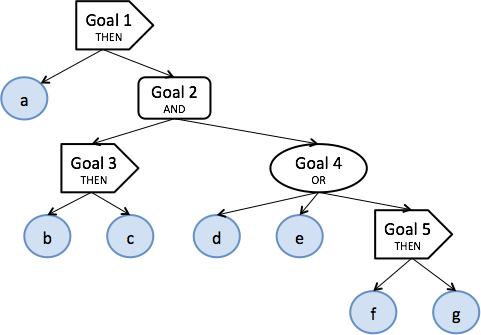
\includegraphics[width=6cm]{task_img}
\caption{Representation of task ``a {\bf THEN} ((b {\bf THEN} c) {\bf AND} (d {\bf OR} e {\bf OR} (f {\bf THEN} g)))''}
\label{fig:task_representation}       % Give a unique label
\end{figure}
%This needs updating
With these types of components, the above task will be represented as shown in Figure~\ref{fig:task_representation}. A task could have any type of goal node as a root and there is no restriction on which nodes could be parents of others in the hierarchy. It can be seen that this representation compactly encodes all the task constraints, including all possible paths of execution. This is especially important when there are multiple alternative paths, such as for Goal2: either Goal3 or Goal4 could be performed first; to achieve Goal4, either one of d, e or Goal5 could be executed. Instead of explicitly enumerating all possibilities \cite{Hawkins2014}, we use the most compact form of the task representation. This representation would be more accurately represented by the following prefix encoding: (THEN a, (AND (THEN b c) (OR d e (THEN f g)))).

\subsection{Task Execution}
\label{execution}

The control architecture operates in a publish and subscribe environment provided by ROS \cite{288}. This facilitates and maintains network connectivity and sends messages between parent and child nodes. Each parent node is connected to its children and each child is connected to its parent. With these connections, timed messages are sent asynchronously between nodes, allowing each node to run in a distributed fashion in the system.

Each node stores the following information: type ({\bf THEN}, {\bf OR}, {\bf AND}, or {\bf BEHAVIOR}),
{\bf status}, which could be \emph{ACTIVE} (i.e, the node is currently performing work), \emph{DONE} (i.e, the node has completed its task), {\bf activation level}, which is the level of activation the node is receiving from its parent, 
and {\bf activation potential}, which is the node's perceived potential for activation. The {\bf BEHAVIOR} type encapsulates all other non-goal nodes in the system (i.e, a placing behavior would of the {\bf BEHAVIOR} node type).
This state information is used to perform distributed top-down and bottom-up activation spreading.

%Luke: please verify that what I wrote below is correct about the types of messages:
The system uses two types of messages: \emph{control messages}, which are sent from parent nodes to their children and \emph{state messages}, which are sent from child nodes to their parent. Control messages contain the following information: \emph{sender} (the node that sent the message), and \emph{activation level} (the amount of activation that the parent sends to the child with this message). State messages contain the following information: \emph{active status} (true if the child node is currently performing an action, i.e, actuating a robot arm), \emph{done status} (true if the node has finished its actions and achieved its goal), \emph{activation level} (the current activation level of the child node) and \emph{activation potential} (the node's perceived potential for activation).

\emph{Activation level} is the primary mechanism for top-down activation spreading. When the root node sends activation to its children, those children will spread their activation to their children. Each \emph{goal} node will impose a different method to determine which children receive activation and when. The activation levels will spread throughout the system until the task is complete.

\emph{Activation potential} is the primary mechanism for bottom-up activation spreading. It solves a critical limitation of only top-down spreading of activation. It is used to pass real-time information on the feasibility of children behaviors. It is useful when determining which child should be awarded higher activation or be activated first. In the case of an {\bf OR} goal node deciding which child to activate, activation potential can be used to pick the most efficient child node.

To execute a task, control messages are sent from the root node of a given task toward its children. At the same time, each node sends status messages to its parent node. This allows decisions to be made both from a top down perspective of the graph as well as from the bottom up. The different types of goal nodes send activation messages as follows:

\begin{itemize}

\item {\bf THEN} goal nodes evaluate the status of their children in the order given by the sequence and send activation messages to the first child node in the list whose status is not met. Once that child node signals completion the subsequent child will receive activation. The 
%Luke: should this be "activation message" below?
activation level is sent to the first child with a control message.
%Luke: above: what is a state message?
%Luke: below: do we describe how nodes update their activation levels? We should say something like "Each child node will update its activation level at each time-step of its update loop, as described in section XXX."
Each child node will update its activation level at each time-step of its update loop.
%This ensures that the subsequent steps of the task are already primed for execution as soon as the current step is done.

%Luke: these need to be revised to match the way you have implemented them.
\item {\bf OR} goal nodes send activation to the child with the highest activation potential. leaf nodes (basic behaviors) will compute and send their activation potential to their parents at each time step. This allows for opportunistic task execution, in situations in which environmental conditions are met for just one (or some) of the alternative pathways. In case of equal activation levels and applicability conditions, the robot will choose one of the options at random. Once a pathway becomes active (detected through messages from the children), the other children will receive zero activation.

\item {\bf AND} goal nodes send activation messages to all their children equally and at the same time.
\end{itemize}


\subsection{Update Loop}
\label{implementation}
%Luke: this may actually fit under the previous subsection. I don't know if it is not repetitive
%As an example, a \emph{THEN} node spreads activation based on the ordering of its children. In the case of the \emph{THEN} node the first child will receive activation prior to the other children. Once the first child signals completion the second child will receive activation. The activation level is sent to the first child with a state message. The child will update its activation level at each time-step of its update loop.


Each node in the system is running an update loop, which runs at every clock tick, and is responsible for controlling the state and the execution of that node. In order to decide a node's actions, the update loop runs through a series of checks, as shown in Algorithm~\ref{update-loop}. All behaviors implement the same update loop as follows:

\begin{itemize}

  \item \textbf{If-Done}: Check if the node has completed its task; if yes, do nothing.
  \item \textbf{If-Active}: Check if the node is active; if not, do nothing.
  \item \textbf{If-Preconditions}: Check if the nodes' preconditions are satisfied; if yes, activate the node, otherwise spread activation (as described below). Preconditions are the set of conditions that must be met in order for the node to begin its work and they ensure that this happens only after all the required tasks constraints are satisfied.
\end{itemize}
  % Luke: this detail should be moved somewhere else, or just cut:
  %In the case of the \emph{THEN} node, All of its children must be complete before the precondition is satisfied. In the case of the \emph{pickup bowl} behavior a mutex must be acquired before work may be done.
  
  Based on the results of the above checks, the nodes may take the following actions:
  \begin{itemize}
  \item \textbf{Activate}: When all the checks are satisfied, the node will activate itself and proceed to perform work. 
  %Luke: above, it is not clear what "perform work" means: is it that it will begin to run an update loop or what in particular? What does this "work" mean for a goal behavior?
  This action signals a thread to begin performing a given node's corresponding behavior. The node will continue to run its update loop unhindered. The work being done is encapsulated by the behavior. In the case of a pick and place behavior performing work is achieved by taking control of robot arm and picking up and placing and object
  .
Each {\bf BEHAVIOR} node's activation is restricted by a mutex, which controls the access to the robot effectors. To become active each node must satisfy a precondition of acquiring the mutex responsible for arm manipulation. The method of acquiring the mutex relies on the behavior's activation potential. When multiple {\bf BEHAVIOR} nodes race to acquire the mutex, access will be given to the node with the highest activation potential. This is accomplished as follows: when the mutex receives a lock request, a timer is started to allow other behaviors to bid for control. When the timer ends the mutex grants the lock to the node with the highest activation potential and denies all other behaviors. The denied behaviors will continue to request a lock until it is acquired. This mechanism enforces responsible use of the robots actuators, as no two behaviors can attempt to use a robot's arm at the same time. As well this locking mechanism can be expanded to allow for further modularization of the robots actuators: one mutex for each arm on the PR2 would allow for actions to be performed in parallel, using both arms.
  
  
  %Luke: for the activation process, we need to say something about the magnitude of the activation message and how it is computed and maintained at each tick
  \item \textbf{Spread Activation}: When the preconditions are not met a control message with an activation level is sent to the children behaviors (as described above). Children nodes do not become active unless their activation level is above a threshold. This threshold is a parameter set at run-time.
  
  %Luke: we need to say something about how the activation level is decreased
  \item \textbf{Activation Falloff}: The activation level of the node is decreased by a prescribed amount at each time-step of the node. This ensures that a node that does not receive activation from a parent will slowly lose activation. The activation level is multiplied by an $\alpha$ value parameter at each time-step of the the update loop. This value is the range between \(0,1\) exclusive.
  \item \textbf{Publish Status}: A status message is sent to the parent at the end of each update loop. This message encodes the current state of the node, which could be \emph{ACTIVE} or \emph{DONE}. 
  %Luke: above, we need to say which are all the possible node states we could have
\end{itemize}

%Luke: It seems like the Activate stage can fail, if the mutex is already taken. We must update the algorithm figure to indicate what happens in that case. 
\begin{algorithm}
\caption{Behavior update loop}
\label{alg:update}
\begin{algorithmic}
\IF {$Not~Done$}
  \IF {$Is~Active$}
    \IF {$Preconditions$}
      \STATE $Activate:$
        \STATE $~~~Mutex Acquired \Rightarrow state \leftarrow active$
    \ELSE
      \STATE $SpreadActivation$
    \ENDIF
    \STATE \emph{ActivationFalloff} $\Rightarrow \alpha ~*$ \emph{activation\_level}  
  \ENDIF
\ENDIF
\end{algorithmic}
\label{update-loop}
\end{algorithm}


%\subsubsection{Goal Nodes}
%\label{sub:sub:actionbehaviors}

%\subsection{Behavior State}


%%%%%%%%%%%%%%%%%%%%%%%
%To perform a task, a robot would use the above task representation as follows: the root node of the task (typically a goal node) receives activation to begin. Each node runs through a checklist during each cycle to determine the current state and actions to perform. This cycle is called the \textbf{Update Loop}:
%\begin{itemize}
%\item \textbf{Check if Done}: If the node is done then there are no more actions to perform.
%\item \textbf{Check if Active}: If the node is active it is receving adequet activation from its parent node to operate.
%\item \textbf{Check Preconditions}: If preconditions are satisfied it is safe for the node to perform work.
%\item \textbf{Spread Activation}: Spread activation levels to children nodes.
%\item \textbf{Activation Falloff}: At each timestep of a node the activation level is reduced by a function. This allows a slow decay of activation if activation is lost from parents. This is to prevent ocilations in actions.
%\end{itemize}

%%%%%%%%%%%%%%%%%%%%%%%

%Luke: I don't know if we can/should use some of the text from the paragraph below. Some of it is duplicate, and some is conflicting with other things we said above...
%Each cycle evaluates the criteria of the update loop to determine the actions of the node. The node is done when its work has been completed successfully. Preconditions are met when all child nodes have completed their work and are done. If all children have completed their tasks, nothing needs to be done. Otherwise, the node will send activation messages to its children nodes in order to signal that they should be met. These goal nodes, in turn, send activation messages as needed to their children. Messages are also passed from children nodes that are currently active (basic behaviors that are running, or goal nodes that are actively being pursued) upwards to the parents to indicate that the current goal is under execution. This is important for keeping track of which pathways of execution and goals are currently under execution and is a key feature that enables seamless self-organization within the robot team. 



\subsection{Progress Checking} 

When a {\bf BEHAVIOR} node's preconditions are satisfied the node's corresponding action will start. The actions are specific for any individual behavior, but the node structure generalizes to any task. In the case of the table setting scenario a \emph{pick-place-cup} behavior is responsible for moving the arm of the robot to the location of the cup and closing the gripper. This action is time-extended and will occur over the span of several seconds. If the state of the environment were to change during this time the execution of the behavior would fail. The progress checking module is responsible for checking the validity of the environmental state during the behavior execution and signalling a reset of the behavior when errors occur. In the case of grasping a cup from the table, the progress checking will monitor the location of the cup and determine if it has changed position during grasp planning. If a significant environmental state change occurs, a signal is sent to stop the behavior's execution and reset the state of the behavior.


\section{Experimental Evaluation}
\label{evaluation}

We evaluated our work using a PR2 humanoid robot working on the task of setting up a dinner table. The objects that the robot can use for this task include: fork, spoon, knife, wine glass, cup, soda can, place mat, plate, and salad plate. We created a task representation that encapsulates all the constraints that occur in such a scenario, as shown in Figure~\ref{fig:set_table}. 

\begin{figure}
\centering
  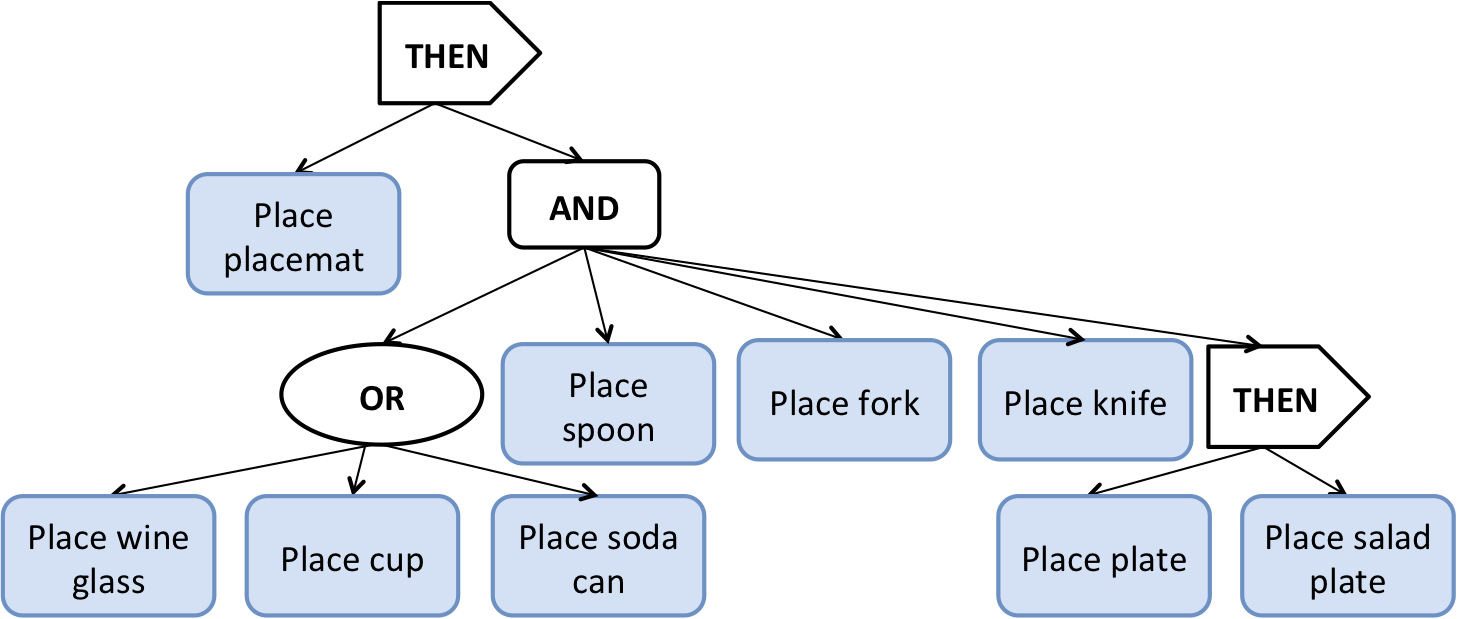
\includegraphics[width=6cm]{set_table_task}
\caption{Task representation for setting up the table}
\label{fig:set_table}       % Give a unique label
\end{figure}

As shown, the task structure encodes sequential constraints (e.g., setting up the place mat before the plate), alternative paths of execution (e.g., choose either the wine glass, the cup or the soda can) and steps whose ordering is not important (e.g., placing the spoon, the fork and one of the drinking objects). For evaluation, we created three different setups, in which the objects are placed at different locations on the table. At execution time, the robot uses the locations of the objects and its activation spreading mechanism to dynamically decide which parts of the task to perform. As currently implemented, the objects that are closer will have a higher activation level than objects farther away, so the robot will choose to first handle the objects that are at a smaller distance, while still maintaining the ordering constraints represented in the task structure. Figure~\ref{fig:setup} shows our experimental environment.

%Luke: take a picture of the environment, for the 3 different setups and include it here
\begin{figure}
\centering
  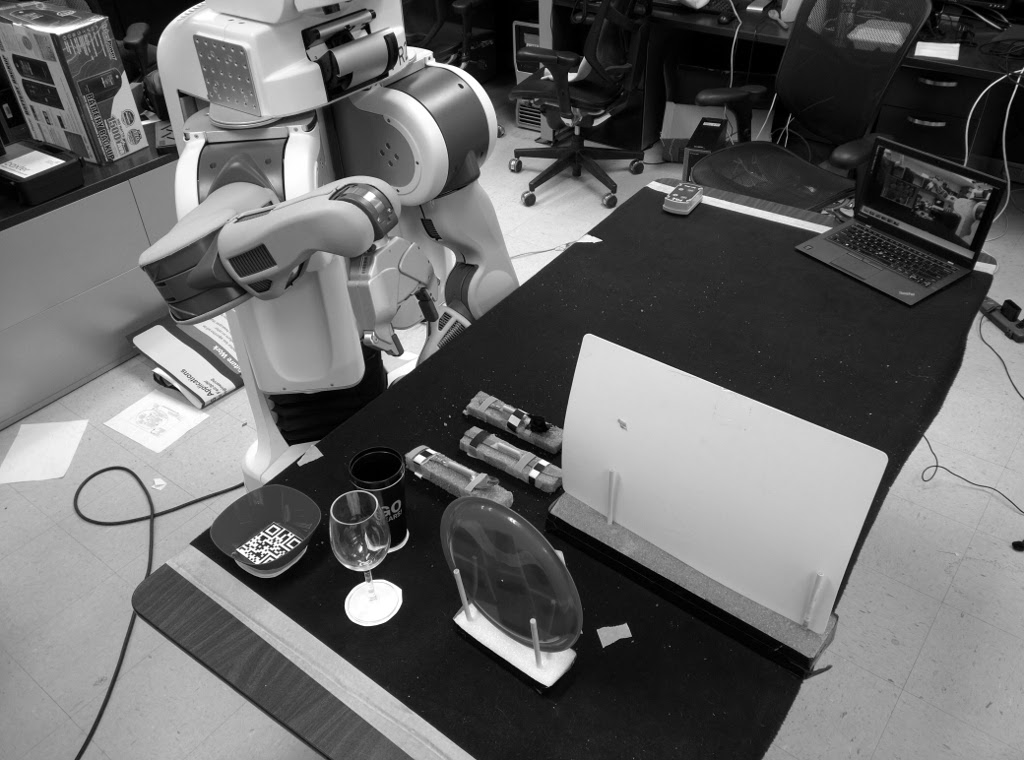
\includegraphics[width=6cm]{bw_task_environment}
\caption{Experimental setup}
\label{fig:setup}       % Give a unique label
\end{figure}


For each experiment we recorded the following information: 1) the activation level for each low-level behavior throughout the duration of the experiment and 2) the times during which the behaviors were active. Figure~\ref{fig:results} show the results of one of the three scenarios. As seen from the plots with the activity of behavior, the robot chooses different ways of achieving the same task, while obeying the constraints set in the task representation. The results show that with the same compact network structure, solely through the activation spreading mechanism, the robot can select its own way of accomplishing the task.

%Luke: I thought we can structure this as a 2 row by 3 column matrix: top row shows the activation levels, bottom row shows the behaviors running
\begin{figure}
\centering
  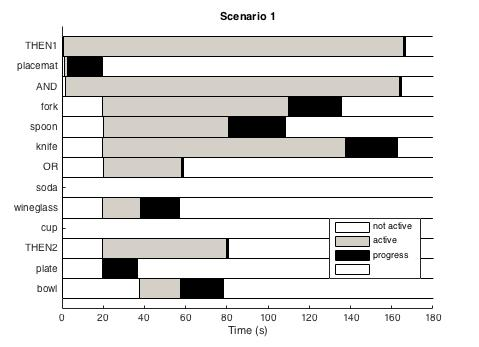
\includegraphics[width=6cm]{scenario1}
\caption{Results from one of the experimental setups showing the run-time decisions.}
\label{fig:results}       % Give a unique label
\end{figure}
\begin{figure}
\centering
  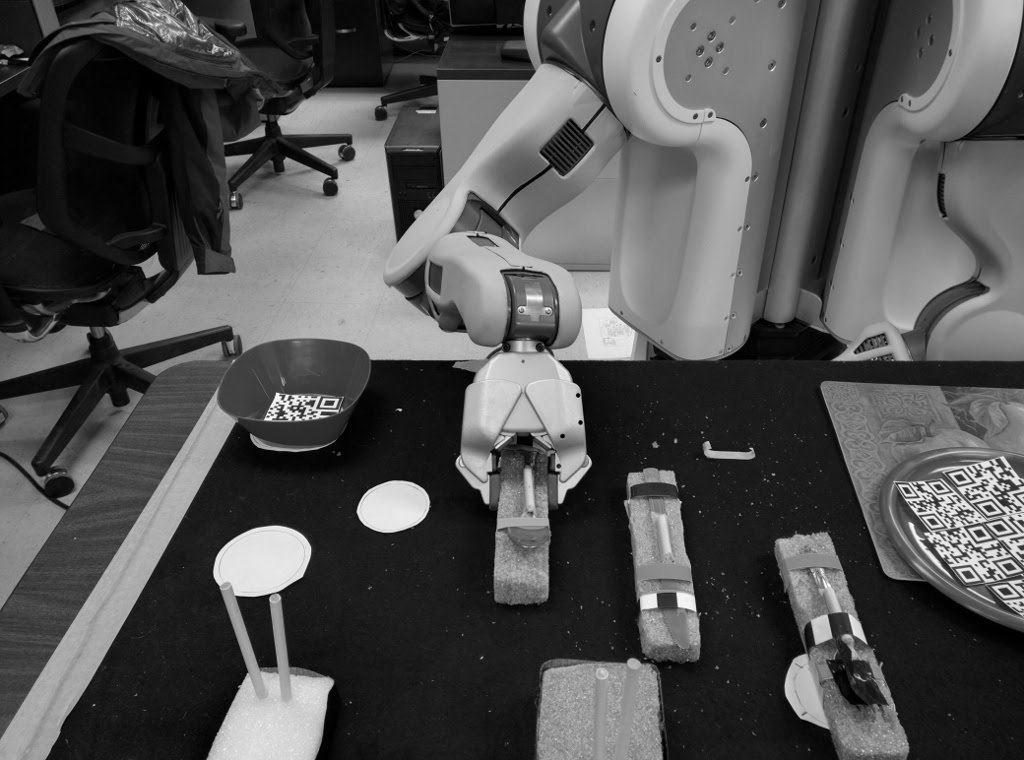
\includegraphics[width=6cm]{environment}
\caption{Stage from task execution}
\label{fig:task-execution}       % Give a unique label
\end{figure}
%Luke: since we have space, we can have a large figure with snapshots from relevant moments in the task execution (e.g. after each object gets picked up) for one of the scenarios. I am adding text for that, we just need to put in the image.

Figure~\ref{fig:task-execution} shows a stage of the task execution for Scenario 1. 

%Luke: need to fix the caption below to fit the scenario


% To demonstrate the robustness of the architecture, we performed experiments in which we interfered with the robot's execution, by moving some of the objects during the time when the robot was trying to reach for them and grasp them. The progress checking mechanism described above detected the change, stopped the currently running behavior and selected a different course of action for the task. This is shown in the behavior activation diagram in Figure~\ref{fig:robustness}, where behavior XXX was stopped before completion, the robot switched to behavior YYY and then behavior XXX was completed at a later time.
%Luke: above, replace XXX and YYY with the corresponding behaviors


\section{Conclusion}
\label{conclusion}
In this paper we presented a new control architecture that allows for efficient encoding of tasks with multiple paths of execution. The representation used for encoding the task structure serves at the same time as a controller that the robot can use for executing the task. Based on this task representation and an activation spreading mechanism within the nodes of the task, the robot can dynamically select which path of execution to perform, based on the current environmental conditions. We validated our approach on a physical humanoid PR2 robot, working on the task of setting the table, in different scenarios that resulted in different ways of execution for the task. Furthermore, we also showed that the architecture is robust to failure when environmental changes are occurring during task execution, enabling the robot to pursue alternative ways of executing the task.
\section*{Acknowledgments}


% \appendix

%% The file named.bst is a bibliography style file for BibTeX 0.99c
\bibliographystyle{named}
\bibliography{refs/master.bib}

\end{document}

\grid
